\documentclass{whutmod}
\usepackage{metalogo}
\usepackage{float}
\usepackage{subfigure} 
\usepackage{url}
\usepackage{booktabs}
\bibliographystyle{unsrt}
\team{23}
\membera{刘子川}
\joba{编程}
\memberb{程宇}
\jobb{建模}
\memberc{陈荣兴}
\jobc{建模}
\hypersetup{
	colorlinks=true,
	linkcolor=black
}

\title{基于因子分析与灰色关联分析对武汉市人才吸引力的量化评价}
\tihao{4} 

\begin{document}

	%\maketitle
	
	\begin{abstract}


%针对问题一,通过\textbf{因子分析模型}分析武汉2013—2017年相关数据,对武汉各年的人才吸引力进行\textbf{量%化打分}。本组首先根据题目要求和以往人才吸引要素研究,确立要素框架并\textbf{爬取}合适的人才吸引力因素。%%转后因子荷载矩阵并对公因子命名,计算武汉各年人才吸引力综合得分。综合得分结果为\textbf{-77.99、-30.08、-%11.90、42.35、77.63}。综合得分表明武汉2013—2017人才吸引力逐年上升,且2015—2016年上升幅度最大,与城市实%际发展情况相符合。
针对问题一,通过\textbf{解析几何计算}和\textbf{时间序列展开},分别提取每一张图片中的特征向量。根据题目要求,本组首先利用matlab计算与图像形状相关的解析几何特征量,得到由八个几何学、拓扑学特征值组成的\textbf{八维}形状特征向量。然后将图像轮廓进行极化投影,并通过numpy工具箱将极化投影轮廓展开成时间序列,挖掘分析时间序列的三个特征值,组成\textbf{三维}边缘特征向量。最后合并两个向量得到\textbf{十一维}总体特征向量。


~\\

针对问题二,本文
~\\

针对问题三,基于问题一中的武汉市人才吸引力评价模型以及人才政策对人才吸引力的量化评价,并结合问题二中武汉相较于其他四个同类城市在人才吸引力上的优势与不足,给武汉市人力资源管理部门的领导写一篇建议报告。
~\\

本文中所提到的模型优点主要有两点:一、选取的指标从多维度、全方面考虑,收集的数据真实可靠;二、利用灰色关联度筛选出三类人才的人才吸引力要素,相较于人工选取指标具有客观性、严谨性。
  
\keywords{因子分析模型\quad  主成分分析\quad  灰色关联分析\quad 数据库爬虫\quad }
		
	\end{abstract}
	
	%目录
	\tableofcontents
	\newpage	%换页符
	
	\section{问题重述}	
	\subsection{问题背景}
    植物的种类繁多,要了解和掌握如此多的植物,必须进行一个科学的分类。人们常常根据植物的用途,或根据植物的一个或几个明显的形态进行分类,植物的识别与分类对于区分植物种类,探索植物间的亲缘关系,阐明植物系统的进化规律具有重要的意义。因此植物分类学是植物科学甚至整个生命科学的基础学科。目前对于树叶识别与分类主要由人完成,但是树叶种类庞大,依赖人工地进行树叶识别与分类是不现实的。所以树叶的研究对于植物总体的研究能提供很大的帮助。
    
    从树叶的各个方面,纹理,硬度,离心率等方面都可作为主要方向研究,现对树叶的研究主要通过采集树叶图形,利用数字图像处理来对树叶进行分类识别,这种方法只停留在处理形态特征,有很大的局限性,忽略了树叶的生理特征和其他特征,所以研究方法来综合处理树叶平面图像特征,形态特征和生理特征很有必要性。
    
    

	\subsection{问题提出}
    围绕植物分类进行树叶识别与分类,以树叶二值化图片为依据,依次提出以下问题:
		 
	\begin{itemize}
	\item [(1)] 结合附件中的二值化的图片数据,建立合适的图片数据提取方案, 量化处理图片数据,并具体分析说明所提取数据信息的量化指标体系。
	\item [(2)] 基于问题一中提取的数据信息,建立合适的数学模型由数据出发判断叶子的种类,研究判别分类的核心指标,并估计出模型的性能以及核心指标对模型判别性能的影响。
	\item [(3)] 基于二值化图片数据,结合附件中叶子纹理的数据信息,对原有模型进行改进,并对新旧模型进行比较分析。
	\end{itemize}
	
	\section{模型假设}
	\begin{itemize}
		\item [(1)] 为保证分类方法具有可推广性,假设现实中同种类树叶与题目所给的树叶二值化图像具有相似的形状轮廓。
		\item [(2)] 人才会考虑未来一段时间内自身对于发展前景、收入、环境的需求的变化。
		\item [(3)] 政策对人才吸引力的影响转换成三个影响因素——地方财政支出与收入和固定资产投资总额。
		\item [(4)] 人才的迁移是在追求效用最大化,人才的行为仅受到城市因子的影响,忽略人的非理性行为。
	\end{itemize}
	
	
	\section{符号说明}
%	每行都有线的表
%	\begin{center}
%		\begin{tabular}{cc}
%			\hline
%			\makebox[0.3\textwidth][c]{符号}	&  \makebox[0.4\textwidth][c]{意义} \\ \hline
%			$C_{0}$	    &  污染源初始浓度 \\ \hline
%			$C(x,t)$	    &  污染浓度随时空变化 \\ \hline
%			$u_{x}$	    &  江河平均纵向流速 \\ \hline
%			$E_{x}$  &  铊在江河纵向弥散系数\\ \hline
%		$p$   &  面污染物纵向距离\\ \hline
%			$K_{c}$	    & 污染物降解系数  \\ \hline
%		    $a$	& 污染超标系数 \\ \hline
%		     $x$	& 距污染源的一维距离 \\ \hline
%		      $t$	& 距污染发生后的时间 \\ \hline
%		       $V_{A}$	& 溶液摩尔体积 \\ \hline
%		      $M_{B}$	& 江水的摩尔质量 \\ \hline
%		     $\mu_{B}$	& 溶剂的粘度 \\ \hline		      
%		\end{tabular}
%	\end{center}

%三线表
	\begin{table}[H]
	\label{biao} \centering
		\begin{tabular}{cc}
			\toprule[1.5pt]
			\multicolumn{1}{m{5cm}}{\centering 符号} & \multicolumn{1}{m{5cm}}{\centering 说明} \\
			\midrule[1pt]
			$F$	 &  城市各年人才吸引力综合得分  \\ 
			$F_{1}$ &  工业发展与薪酬因子 \\ 
			$F_{2}$	 &  医疗卫生环境因子 \\ 
			$F_{3}$  &  经济贸易因子 \\ 
			$F_{4}$  &  拥挤程度因子 \\ 
			$X$  &  原始指标 \\ 
			$\overline{X}$  &  指标平均值 \\ 
			$\widetilde{X}$  &  同向化指标 \\ 
	     	$\delta_{X}$  &  指标标准差 \\ 
	     	$Z$  & 标准化指标 \\ 
	     	$R$  & 相关系数矩阵 \\ 
	     	$\lambda_{p}$  & 相关系数矩阵特征值 \\ 
	     	$\eta _ {p}$  & 标准正交化特征向量 \\ 
	     	$\Lambda$ & 因子载荷矩阵 \\ 
	     	$\sigma_{i}$ & 方差 \\
	     	$\alpha_{i j}$ & 载荷因子 \\
	     	$k$ & 两极最小差 \\
	     	$K$ & 两极最大差 \\
	     	$\Delta _{i}(t)$ & 特征序列与因素序列的序列差 \\
			\bottomrule[1.5pt]
		\end{tabular}
	\end{table}

	\section{问题一模型的建立与求解}
	\subsection{问题的描述与分析}

	针对问题一,本题要求建立合适方案提取二值化图片中的数据,并对所提取数据的量化指标进行分析说明。本组通过解析几何计算和时间序列展开,将目标图像转化成两个特征向量。本组根据题目要求和近年的图像识别研究,确定了针对二值化图像的两个重点识别因素——形状特征因素和边缘特征因素。针对形状特征因素,首先利用matlab做解析几何运算,计算与图像轮廓有关的特征量,并将计算结果作为元素,组成轮廓特征向量。针对边缘特征因素,首先将图像边缘通过极化投影展开为时间序列,计算每支时间序列的特征量,并将计算结果作为元素,组成边缘特征向量。最后合并两个向量得到总体特征向量。其具体特征值如图~\ref{77}~所示:
	    \begin{figure}[H]
		\centering
		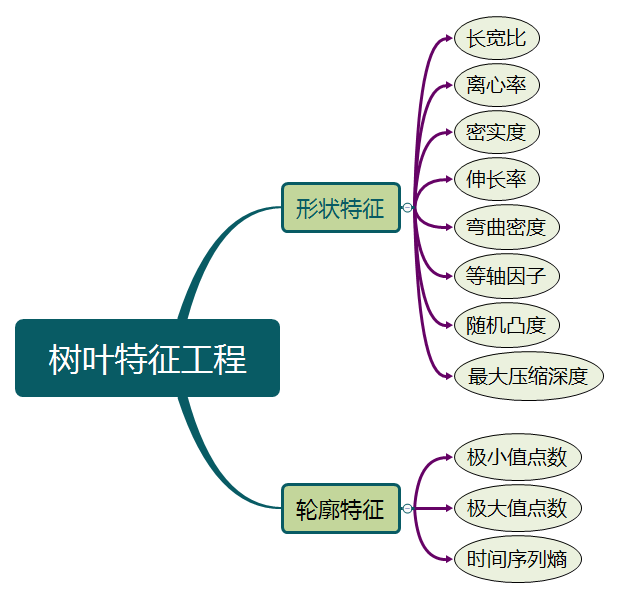
\includegraphics[width=.6\textwidth]{figures/flt.png}
		\caption{图形特征示意图}\label{77}
    	\end{figure}
	
	    \subsection{模型的建立}
	    \subsubsection{图像基本参数与运算符号定义}
		定义$I$表示目标树叶所对应的图像,$\partial I$表示图像边界,$D(I)$表示图像最小外接圆直径,$d(I)$表示图像最大内切圆半径,$A(I)$表示研究对象面积,$L(\partial I)$表示研究对象的轮廓线长度,$H(I)$表示研究对象的凸包域,$C(I)$为图像几何中心坐标,运算符$d(.)$代表欧式距离。

	    \subsubsection{形状特征因素}
		定义轮廓特征向量为$ID_{shape}=[id_{1},id_{2},\cdots,id_{n}](n=6)$其中$id_{k}(k=1,2,\cdots,6)$为二值化矩阵的轮廓特征,其具体计算公式如下:
		\begin{itemize}	
		\item [(1)]长宽比(Aspect Ratio):
		定义$X_{I}$为图像最上方非零行与最下方非零行的行数差(长),$Y_{I}$为图像最左方非零列与最右方非零列的列数差(宽),即长宽比计算公式:
		\begin{gather}
		id_{1}=X_{I}/Y_{I}
		\end{gather}

		
		\item [(2)]离心率(Eccentricity): 
		定义$E(I)$是与研究图像具有相同的二阶矩的椭圆,$a$和$b$分别为$E(I)$对应的长轴与短轴,即离心率计算公式:
		\begin{gather}
		id_{2}=\sqrt{1-(\frac{b}{a})^{2}}
		\end{gather}
		
		
		\item[(3)]密实度(Solidity):
		反映研究对象的仿射特征的变量,即研究对象区域的固靠性程度,计算公式:
		\begin{gather}
		id_{3}=\frac{ A }{A(H(I))}
		\end{gather}
		
		\item [(4)]等周因子(Isoperimetric Factor):
		描述目标树叶轮廓规整度的变量,变化范围为(0,1),叶子边缘越规则,其值越接近于最大值1,计算公式:
		\begin{gather}
		id_{4}=\frac{4\pi \cdot  A}{L(\partial I)^{2}}
		\end{gather}
		
		\item [(5)]伸长率(Elongation): 
		描述研究对象向某方向伸展趋势的变量,变化范围为(0,1),树叶越趋于圆形相应的伸长率越小,计算公式:
		\begin{gather}
		id_{5}=1-\frac{2d_{I}}{D(I)}
		\end{gather}
		
		\item[(6)]最大压痕深度(MaximalIndentationDepth):
		定义$C_{H(I)}$为研究对象凸型区域的几何中心,$L(\partial I)$表示为$H(I)$的轮廓线长度,$\forall X\in H(I)$和$\forall Y\in \partial I$,计算距离$d(X,C_{H(I)})$和$d(Y,C_{H(I)})$。即最大压痕深度计算公式为:
		\begin{gather}
		max\left \{ \frac{ d(X,C_{H(I)})- d(Y,C_{H(I)})}{L(H(I))} \right \}
		\end{gather}
		
		\item[(7)]随机凸性(Stochastic Convexity):
		记随机给定两个端点$P_{1},P{2}\in\partial I$,记$P(G)$为线段$[XY]$完全包含于图像区域$I$ 中的概率,即随机凸性计算公式为:
		\begin{gather}
		id_{7}=P(G)
		\end{gather}
		
		\item[(8)]弯曲能量(Bending Energy):
		描述研究对象边界弯曲程度的值,定义$\varphi _{n}$为$\partial I$的曲率,即弯曲能量计算公式为:
		\begin{gather}	
		id_{8}= 1 / P \sum _ { i = 0 } ^ { n - 1 } \left|\varphi _{n} -\varphi _{n-1}\right|
		\end{gather}
		
		
		
		
		
		\end{itemize}	

	

		\subsubsection{边缘特征因素}
		为得到研究对象的边缘特征,首先以$C(I)$为坐标原点建立笛卡尔坐标系,对于曲线$\partial I$上任意一点$P$可以在该坐标系下表示为$P(x_{p},y_{p})$,将其投影至以$C(I)$为极点的极坐标系得${P}'(r_{p},\theta _{p})$,其中:
		\begin{gather}
		r_{p}=d(P(x_{p},y_{p}).C(I))
		\end{gather}
		\begin{gather}
		\theta _{p}=y_{p}/x_{p},
		\end{gather}

	  \begin{figure}[H]
		\centering
		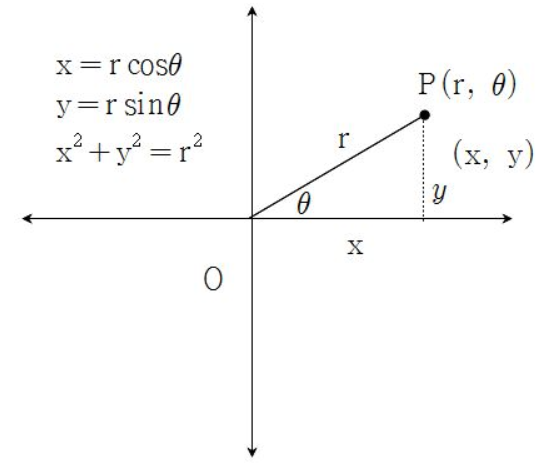
\includegraphics[width=.6\textwidth]{figures/jihua.png}
			\centering 		\caption{极化投影实意图}\label{66}
	\end{figure}
		
		定义点集${{P}'(r_{p},\theta _{p})}$为研究样本,其中中包含${d}'$个一元时间序列,$Q$为单个样本一维的长度。将数据集中每个样本第$j$维$(j\in \left \{1,2,\cdots,d  \right \})$数据组成一个一元时间序列数据集,记为$X$。且
		其中表类样本$y _ { i } \in \{ 1,2 , \cdots , C \} , i \in \{ 1 , \cdots , N \}$。
		
		得到一元时间序列集$X$后,记$N$为序列集中的时间序列条数。在数据集$D$中有$n_{i}$个实例,并且$n_{1}+n_{2},\cdots,n_{n}=N$计算$X$序列集熵值作为边缘特征值:
		\begin{gather}
		id_{9}= - \sum _ { i = 1 } ^ { C } \frac { n _ { i } } { N } \log \frac { n _ { i } } { N }
		\end{gather}
		
		定义$shapelet$为时间序列$X$中能够最大程度区分不同类别时间序列的子序列。在一元时间序列分类问题中选出$K$个最优shapelet并记为$S\in R^{K\times M}$(其中M为shapelet的长度。一个长度为M的shapelet
		\begin{gather}
		S_{k}=\left\{ s _ { k 1 } , s _ { k 2 } , \cdots , s _ { k n } \right\} ( k \in \{ 1 , \cdots , K \} )
		\end{gather}
	
		是时间序列$X_{i}(i\in \left \{1,2,\cdots,d  \right \})$的子序列,定义$X_{i}$与$S_{k}$之间的距离为:
		\begin{gather}
		D _ { i , k } = \min _ { j = 1 , \cdots , j } \frac { 1 } { M } \sum _ { m = 1 } ^ { M } \left( X _ { i , j + m - 1 } - S _ { k , m } \right) ^ { 2 }
		\end{gather}
		其中$M$表示所选定的$X_{i}$与$S_{k}$的子序列长度。再找到在找到$K$个最优shapelet后,计算$K$个最优shapelet与一个时间序列间的距离作为该时间序列的新特征,时间序列样本集被映射至新特征空间,最终将之间序列降至一维时间序列arrays,展开效果如图~\ref{99}~所示:
					\begin{figure} [H]
			\centering 
			\subfigure[Acer-Campestre]{% 
				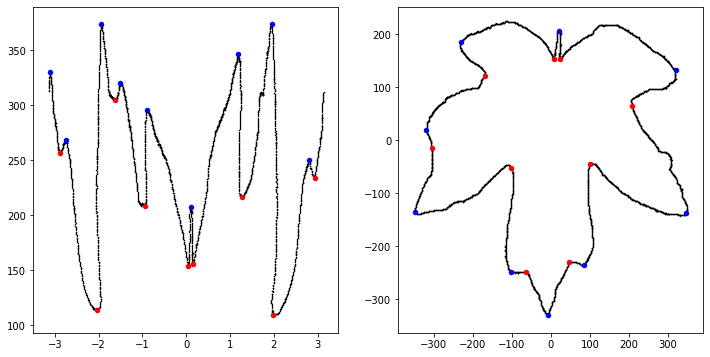
\includegraphics[width=\textwidth]{figures/sjxl.png}}
			\quad
			\subfigure[Cornus-Controversa]{% 
				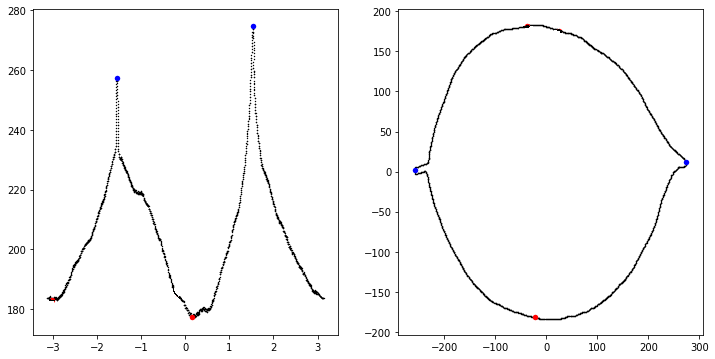
\includegraphics[width=\textwidth]{figures/sjxl2.png}}
				\caption{时间序列展开效果图}\label{99}	
		\end{figure}

	
		将arrays滤波处理后,计算每支时间序列上的极大值点数$id_{10}$,极小值点数$id_{11}$。得到边缘特征向量$ID_{margin}=[id_{9},id_{10},id_{11}]$,合并轮廓特征向量与边缘特征向量得:
		\begin{gather}
		ID=[ID_{shape},ID_{margin}]
		\end{gather}
	     其中ID为总体特征向量。
	      \subsection{模型的求解}
	      首先使用matlab围绕regionprops函数对研究对象进行解析几何计算,用遍历式算法逐一算出研究对象长宽比、离心率、实密度、等周因子、伸长率和最大压痕深度,得到轮廓特征向量。再将图片通过numpy工具箱标准正立化,以其几何中心为极点将其边缘坐标转换为极坐标,然后使用ndarrays函数将所得极坐标降维展开成时间序列,搜寻滤波后时间序列的极点数得到边缘特征向量。其算法流程图如图~\ref{88}~
	      
	      \begin{figure}[H]
	      	\centering
	      	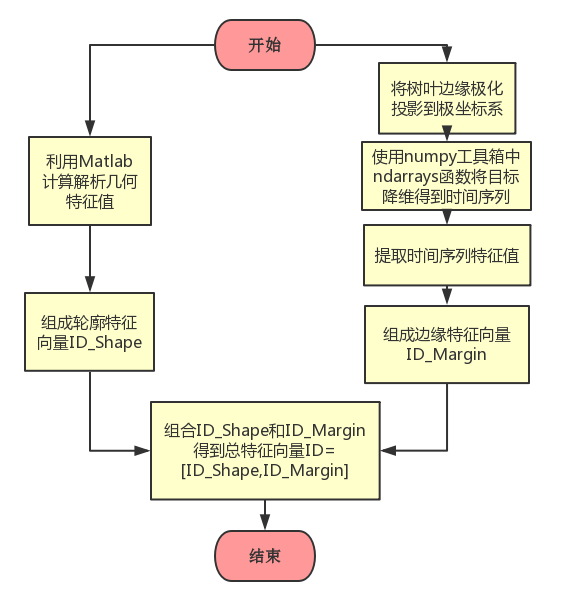
\includegraphics[width=.8\textwidth]{figures/lct.png}
	      	\caption{树叶特征工程示意图}\label{88}
	      \end{figure}
	      	
	
	
	
	
	\section{问题二模型的建立与求解}
	\subsection{问题的描述与分析}
	问题二要求针对所提取数据信息,建立数学模型判别叶子的种类并研究其核心指标。本组通过问题一中所提取的$11$维度的特征,采用$Keras$工具库搭建深度神经网络(DNN)解决树叶多分类问题,并输出各维度特征的权重作为指标贡献率。DNN神经网络采用BP算法基于梯度信息来调整连接权值,因而初始权值和阈值选取的随机性会导致网络稳定性差。为克服此缺点,引入收敛速度快、全局搜索能力强的PSO算法来优化DNN网络的连接权值和阈值,建立一种新的$PSO-DNN$网络模型实现对树叶分类。当考虑到步长等参数的选取时,使用网格搜索的方式对参数进行优化,其流程图如下:
		
	\begin{figure}[H]
	\centering
	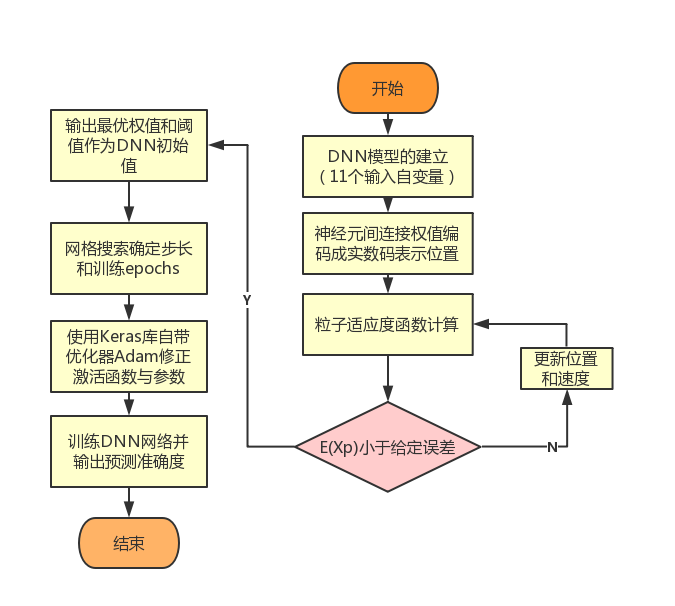
\includegraphics[width=\textwidth]{figures/21.png}
	\caption{PSO算法优化DNN网络流程图}\label{2222}
	\end{figure}


	\subsection{模型的建立与求解}
	
	\subsubsection{DNN网络搭建}
	DNN的正向传播主要依靠众多神经元的计算来完成的,此处设计的网络结构如图~\ref{dnn}~所示,工作过程中可以用下式来表示:
			\begin{gather}
{u_{k}=\sum_{i=1} w_{k i} x_{i}} \\ {y_{k}=f\left(u_{k}-b_{k}\right)}
	\end{gather}
	其中:$x_{i}$表示第 i 个输入; $w_{ki}$表示与第 i 输入量相 连的权值; $u_{k}$表示所有输入的加权和; $b_{k}$为神经 元阈值;$ f$ 为激活函数; $y_{k}$ 为神经网络的输出。
	
	激活函数的种类有很多,如 $sigmoid$, $tanh$ 及$ Relu$,本文应用的是 $Relu$作为激活函数搭建两层隐含层,如式~\ref{shiw}~所示:
	\begin{gather}\label{shiw}
		\begin{array}{c}{f_{\text {Relu}}=\max (0, z)}\\
		\frac{d}{d z} f_{R e L U}=\left\{\begin{array}{ll}{1,} & {z>0} \\ {0,} & {z \leqslant 0}\end{array}\right.
		\end{array}
	\end{gather}
	
	网络的输出层使用$ softmax $函数作分类器, 式~\ref{shiq}~为第 i 个神经的输出:
	\begin{gather}\label{shiq}
		f_{\text {softinax }}=\mathrm{e}^{i} / \sum_{j} \mathrm{e}^{j}
	\end{gather}
	
		\begin{figure}[H]
		\centering
		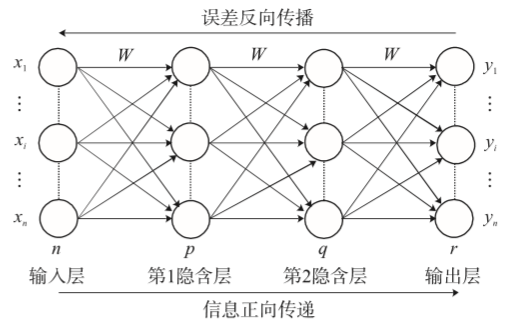
\includegraphics[width=\textwidth]{figures/123546.png}
		\caption{人工搭建DNN结构示意图}\label{dnn}
	\end{figure}
	
	
	\subsubsection{PSO优化DNN网络}
	算法的具体实现步骤如下:
	\begin{itemize}
		\item [(1)]将DNN网络结构中所有神经元间的连接权值和各个神经元的阈值编码成实数码串表示的个体作为PSO算法要寻优的位置向量。
		\item [(2)]在编码空间中随机生成一定数目的个体组成种群,其不同个体代表神经网络不同权值。
		\item [(3)]DNN网络训练及个体的适应度评价。将微粒群中的每一个个体的分量映射为网络中的权值和阈值,从而构成个体对应的神经网络。首先划分训练样本和测试样本;其次输入训练样本进行网络训练,通过反复迭代来优化网络权值,并计算每一个网络在训练集上产生的均方误差,,以此作为目标函数;最后对每个个体进行适应度评价,从中找到最佳个体用来判断是否需要更新微粒的Gbest与Pbest,构造如下的适应度函数:
			\begin{gather}
		E\left(X_{p}\right)=\frac{1}{n} \sum_{p=1}^{n} \sum_{k=1}^{c}\left[Y_{k, p}\left(X_{p}\right)-t_{k, p}\right]^{2}
		\end{gather}
		
		式中:$n$为训练样本个数,
		$c$为输出端个数,$t_{k,p}$为训练样本
		$p$在$k$端的给定输出,
		$Y_{k,p}\left(X_{p}\right)$为训练样本$p$在$k$端的实测值,他们俩个值的误差平方和越小,表示实际值和预测值越接近,网络的性能越好。
		
		\item [(4)]更新每个粒子的速度和位置,产生下一代的粒子群。更新公式如下:
		\begin{gather}
		v_{id}^{t+1}=v_{id}^{t}+c_{1}r_{1}(p_{id}^{t}-x_{id}^{t})+c_{2}r_{2}(g_{id}^{t}-x_{id}^{t})
		\end{gather}	
		\begin{gather}
		x_{id}^{t+1}=x_{id}^{t}+v_{id}^{t+1}
		\end{gather}
		其中$i=1,2,...,n$;$d=1,2,...,d$;$t$为当前迭代次数;$v_{id}^{t}$为当前粒子速度($t$时刻);$x_{id}^{t}$为当前粒子位置($t$时刻);$(p_{id}^{t}-x_{id}^{t})$为当前位置与自己最好位置之间的距离;$(g_{id}^{t}-x_{id}^{t})$为当前位置与群体最好位置之间的距离;$v_{id}^{t+1}$为下一时刻粒子速度($t+1$时刻);$c_{1},c_{2}$为非负常数,称为加速因子;$r_{1},r_{2}$为均匀分布与$[0,1]$区间的随机数。
		
		\item [(5)]当目标函数小于给定的误差或达到最大迭代次数时,算法结束。将PSO算法训练出来的最佳神经网络的权值和阈值作为DNN网络的初始值,并记录。
		
	
	\end{itemize}
	
	\subsubsection{参数的选取与确定}
	由于训练epochs与步长选取较为困难,实验采取\textbf{网格搜索法}(Grid Search)来确定参数的选取,网格搜索是指定参数值的一种穷举搜索方法,通过将估计函数的参数通过交叉验证的方法进行优化来得到最优的学习算法。
	
	在迭代修正的过程中,实验采用$Keras$自带优化器\textbf{$Adam$函数}进行迭代修正,如式~\ref{adam}~所示,其中$\beta_{1}$一般取0.9,$\beta_{2}$一般取0.999。
	
	\begin{gather*}\label{adam}
	\left\{\begin{array}{l}{m_{t}=\beta_{1} m_{t-1}+\left(1-\beta_{1}\right) \nabla_{w} f\left(w_{t}\right)} \\ {v_{t}=\beta_{2} v_{t-1}+\left(1-\beta_{2}\right) \nabla_{w} f\left(w_{t}\right)^{2}} \\ {\widehat{m}_{t}=\frac{m_{t}}{1-\beta_{1}^{t}}, \hat{v}_{t}=\frac{v_{t}}{1-\beta_{2}^{t}}} \\ {w_{t}=w_{t-1}-\eta \frac{\widehat{m}_{t}}{\sqrt{\hat{v}_{t}+\varepsilon}}}\end{array}\right.
	\end{gather*}


	\subsection{实验与结果分析}
	随机选取80\%的数据作为训练集进行数据\textbf{标准化处理},再对树叶种类(species)进行\textbf{One-Hot编码}作为分类目标。训练输入样本为$1280*11$,测试输入样本为$320*11$,DNN网络输入层神经元$11$个,输出层神经元$100$ 个,包含$2$个隐含层,适应度函数选择均方误差。按照PSO优化DNN网络模型的步骤不断地迭代寻找最优网络参数,进行树叶分类预测的仿真实验。具体参数设置间表~\ref{canshu}~。
			\begin{table}[H]
		\centering		\caption{参数设置表}\label{canshu}
		\begin{tabular}{ccc}
			\toprule[2pt]
			\multicolumn{1}{m{4cm}}{\centering 参数名称}
			& \multicolumn{1}{m{3cm}}{\centering 参数符号}
			&\multicolumn{1}{m{3cm}}{\centering 参数值}
			\\
			\midrule[1pt]
			选择粒子个数为	 &  T &$30$ \\ 
			计算精度	 &  $\varepsilon$&$0.00001$  \\ 
			学习率	 &  $\eta $ &0.01 \\ 
			最大迭代次数	 &  $M$ &500\\ 
						维度	 &  $S$ &11 \\ 
									加速因子1	 &  $c_{1}$ &1.49\\ 
												加速因子2	 &  $c_{2}$ &1.49 \\ 
			惯性权重	 &  $\beta $ &$0.9$ \\ 
			\bottomrule[2pt]	
		\end{tabular}

	\end{table}
	
	通过上述参数设置,训练后各维度权重占比如图~\ref{quanzhong}~所示,最小均方误差为0.458,\textbf{预测准确率为$91.237\%$}。
	其迭代过程中损失与准确率如下图所示:
	\begin{figure}[H]
		\centering
		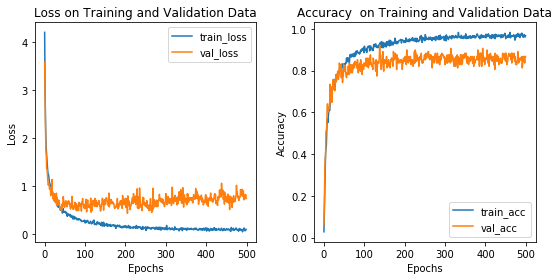
\includegraphics[width=\textwidth]{figures/x.png}
		\caption{PSO-DNN迭代过程中损失与准确率}\label{xxx}
	\end{figure}

	\begin{figure}[H]
	\centering
	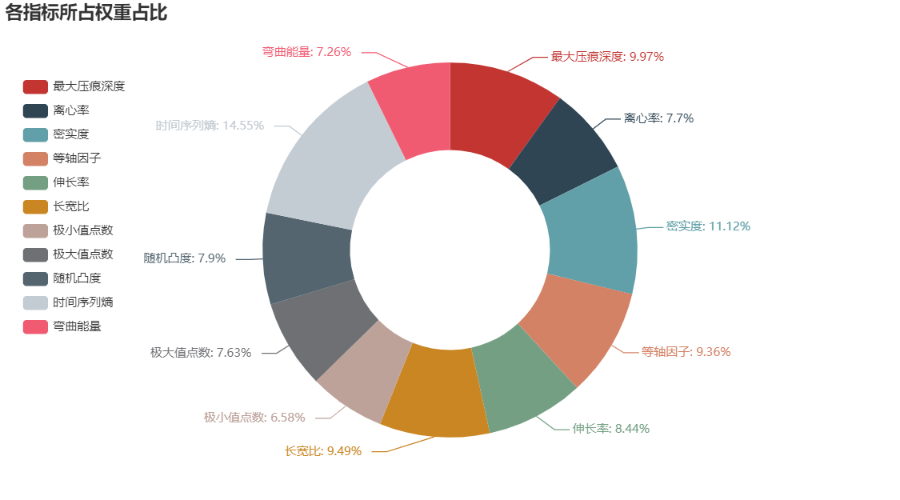
\includegraphics[width=\textwidth]{figures/quanzhong2.png}
	\caption{各维度权重占比图}\label{quanzhong}
\end{figure}
%	从图~\ref{xxx}~可以看出,PSO-DNN网络训练后,在测试集中表现良好效果良好,在
	\subsubsection{模型性能评估}
	表~\ref{heng}~中,实验与三种神经网络进行纵向比较可知,四种神经网络训练后准确率都在90\%左右,证实了神经网络非线性映射能力较强。Elman网络和DNN网络的测试准确率都大于BP网络,说明反馈动态网络的逼近能力要强于前反馈静态网络。使用PSO优化DNN网络后,模型的跟踪性能有所改善,测试集中损失(Validation Loss)仅为0.458,说明PSO-DNN网络的泛化能力和稳定性明显提高,且全局收敛性增强。
	
		\begin{table}[H]
	 \centering	\caption{常见神经网络的比较}\label{heng}
		\begin{tabular}{ccc}
			\toprule[2pt]
			\multicolumn{1}{m{3cm}}{\centering 网络类型}
			 & \multicolumn{1}{m{3cm}}{\centering 网络名称}
			  &\multicolumn{1}{m{4cm}}{\centering 测试集中准确率}
			  \\
			\midrule[1pt]
			静态网络	 &  BP &87.424\%  \\ 
			静态网络	 &  Elman &90.541\%  \\ 
			动态网络	 &  DNN &89.912\%  \\ 
			动态网络	 &  PSO-DNN &91.237\%  \\ 
			\bottomrule[2pt]	
		\end{tabular}

	\end{table}



	\section{问题三模型的建立与求解}
    \subsection{问题描述与分析}
    针对问题三,本题要求结合给出的叶子纹理的数据信息,对问题二原有模型进行改进并进行分析比较。本组
    
	
		
    \subsection{模型的建立与求解}
    
    \subsection{结果分析}
	
	
	\section{模型的评价}
	\subsection{模型的优点}
	\begin{itemize}
		\item [(1)] 从国家统计数据库、武汉市统计年鉴和其他同类城市的统计年鉴中爬取大量数据,并挑选符合实际的33个指标与最近五年的数据进行评价。其吸引人才指标从多维度、全方面的考虑,具备科学性、客观性。
		\item [(2)]针对具体人才根据相应产业进行分类。相较于现有城市人才吸引力水平评价模型,我们采用了灰色关联分析法,对三种人才类别分析计算出与指标的相关系数,求出不同人才对33种影响因素的的偏好程度,选出前十个合适的指标进行综合打分。
	\end{itemize}

	
	\subsection{模型的缺点}
    未能具体地量化政府政策对人口吸引力的影响,只选取了地方财政收入、支出,固定资产投资总额三个影响因素作为政策影响的指标,与现实情况出现一定偏差,存在一定的局限性。

    
    
	\newpage	%换页符
	%%参考文献
	%\begin{thebibliography}{9}%宽度9
	% \setlength{\itemsep}{-2mm}
	\nocite{*}		%排版未引用的参考文献
\bibliography{wenxian.bib}
	%参考文献添加到wenxian.bib里,再引用
	
	\newpage
	%附录
	\appendix %%附录
\section{代码}
\subsection{数据预处理--python源代码}
\begin{lstlisting}[language=python]%这里修改语言
import pandas as pd
from sklearn.preprocessing import StandardScaler
from sklearn.decomposition import PCA
from factor_analyzer import FactorAnalyzer

#导入数据
df = pd.read_excel("wut.xls")
# print(df.head(5))

#转置
df = pd.DataFrame(df.values.T, index=df.columns, columns=df.index)
# print(df['商品房平均销售价格(元/平方米)'])

数据正向处理
df['商品房平均销售价格(元/平方米)'] = -(df['商品房平均销售价格(元/平方米)']-sum(df['商品房平均销售价格(元/平方米)'])/5)
df['工业废水排放量(万吨)'] = -(df['工业废水排放量(万吨)']-sum(df['工业废水排放量(万吨)'])/5)
df['工业二氧化硫排放量(吨)'] = -(df['工业二氧化硫排放量(吨)']-sum(df['工业二氧化硫排放量(吨)'])/5)
print(df['商品房平均销售价格(元/平方米)'])
print(df.head(5))
df.to_excel("武汉.xls")

#数据标准化
df = StandardScaler().fit_transform(df)
# print(df)
df=pd.DataFrame(df)
df.to_excel("武汉.xls")
#
#主成分分析
pca = PCA(n_components=4)
newX = pca.fit_transform(df)
print(newX)

#返回所保留的n个成分各自的方差百分比
print("它代表降维后的各主成分的方差值占总方差值的比例,这个比例越大,则越是重要的主成分")
print(pca.explained_variance_ratio_)
print("它代表降维后的各主成分的方差值,方差值越大,则说明越是重要的主成分")
print(pca.explained_variance_)

\end{lstlisting}


\end{document}